% !TeX encoding = UTF-8
% !TeX program = xelatex
% !TeX spellcheck = en_US

\documentclass{cjc}

\usepackage{cite}
\usepackage{booktabs}
\usepackage{algorithm}
\usepackage{algorithmic}
\usepackage{siunitx}
\usepackage[normalem]{ulem}
\useunder{\uline}{\ul}{}

\classsetup{
  % 配置里面不要出现空行
  title        = {基于SGDRegressor和 LassoCV方法对工业蒸汽量回归预测},
  title*       = {Industrial steam prediction based on SGDRegressor and LassoCV methods},
  authors      = {
    author1 = {
      name         = {李子怡},
      name*        = {Ziyi Li},
      affiliations = {aff1},
      biography    = {},
      biography*   = {},
      email        = {liziyi@hust.edu.com},
      classname    = {自实1801班},
      student-id = {U201814168},  % 学号
    }
  },
  affiliations = {
    aff1 = {
      name  = {华中科技大学,人工智能与自动化学院},
      name* = {School of Articial Intelligence and Automation, Huazhong University of Science and Technology},
    },
  },
  abstract     = {回归预测一直是数据科学的一大热门问题,在这篇文章中,利用阿里云的天池比赛中的工业蒸汽量预测数据集进行回归预测。该数据集一共有三十八个特征,target作为预测目标,以均方误差作为评判标准。本篇文章针对此数据集,进行了数据预处理,加入稳定性判据增强算法的稳定性,在分析使用了效果相对较好的SGDRegressor和 LassoCV方法进行预测。
通过比较测试集和训练集的特征分布差异去掉某些分布差异特别大的特征,通过统计特征重要性来选取特征,对数据进行归一化,同时使用了交叉验证来训练参数,以达到更优的效果,尝试使用Adaboost进行模型融合,尝试了多种模型,在线上测试集最低均方误差为0.1723。
  },
  abstract*    = {Regression prediction has always been a hot issue in data science.  For this data set, this article preprocessed the data, added stability criteria to enhance the stability of the algorithm, and used the relatively good SGDRegressor and LassoCV methods for prediction in the analysis.
By comparing the feature distribution differences between the test set and the training set, some features with very large distribution differences are removed, features are selected by statistical feature importance, the data is normalized, and cross-validation is used to train parameters to achieve better I tried to use Adaboost for model fusion, tried a variety of models, and the minimum mean square error on the online test set was 0.1723},
  keywords     = {回归预测, 特征选择, 线性回归,模型融合},
  keywords*    = {Regression prediction, feature selection, Linear Regression,Adaboost},
}

\newcommand\dif{\mathop{}\!\mathrm{d}}

% hyperref 总是在导言区的最后加载
\usepackage{hyperref}


\begin{document}

\maketitle


\section{介绍}
本文的结构如下。第二节介绍针天池工业蒸汽量数据集进行的预处理过程、讲述了使用的方法、和如何训练模型。第三节给出了实验结果并进行了不同模型间的效果比较。第四节给出了总结。代码和本篇文章中所使用的图可在\href{https://github.com/easilylazy/data-science/tree/main/Zhengqi}{Github}查看。


\section{方法}

\subsection{预处理}

\subsubsection{数据集统计}
该数据集分为训练集和测试集,其中训练集共有2888个样本,每一个样本均有38个特征,经统计均没有缺失值。训练集中给出 'target' 变量作为预测目标。测试集共有1925个样本,每个样本有38个特征,无缺失值。
% \usepackage{booktabs}

\subsubsection{特征选择}
首先我们进行测试集和训练集的样本特征分布比较,观察发现V5、V22分布差异比较大,我们将这几个特征删除作为一种特征提取的方案。
此两个特征的分布如图\ref{fig:distri}:
\begin{figure}[htb]
  \centering
  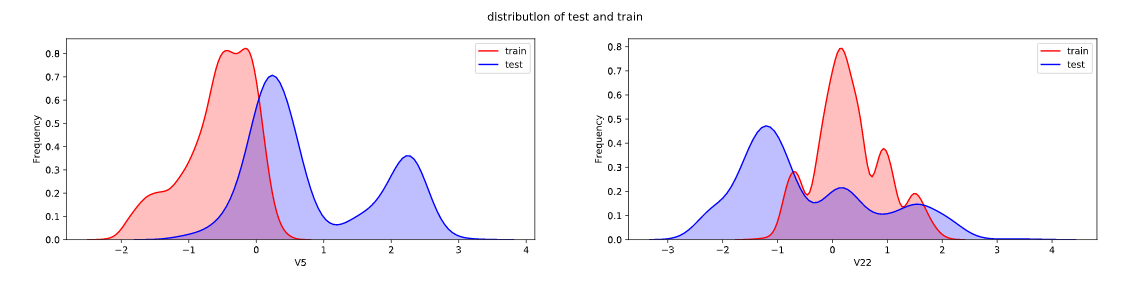
\includegraphics[width=250pt]{fig/distribution.png}
  \caption{删去的两个特征测试集与训练集差异}
  \label{fig:distri}
\end{figure}
此外,还有如图\ref{fig:distri2} V9,V11,V17分布差异较大,这里我们可以进一步删去,但因为可能进一步丢失信息,所以我们将其做为方法二。
\begin{figure}[htb]
  \centering
  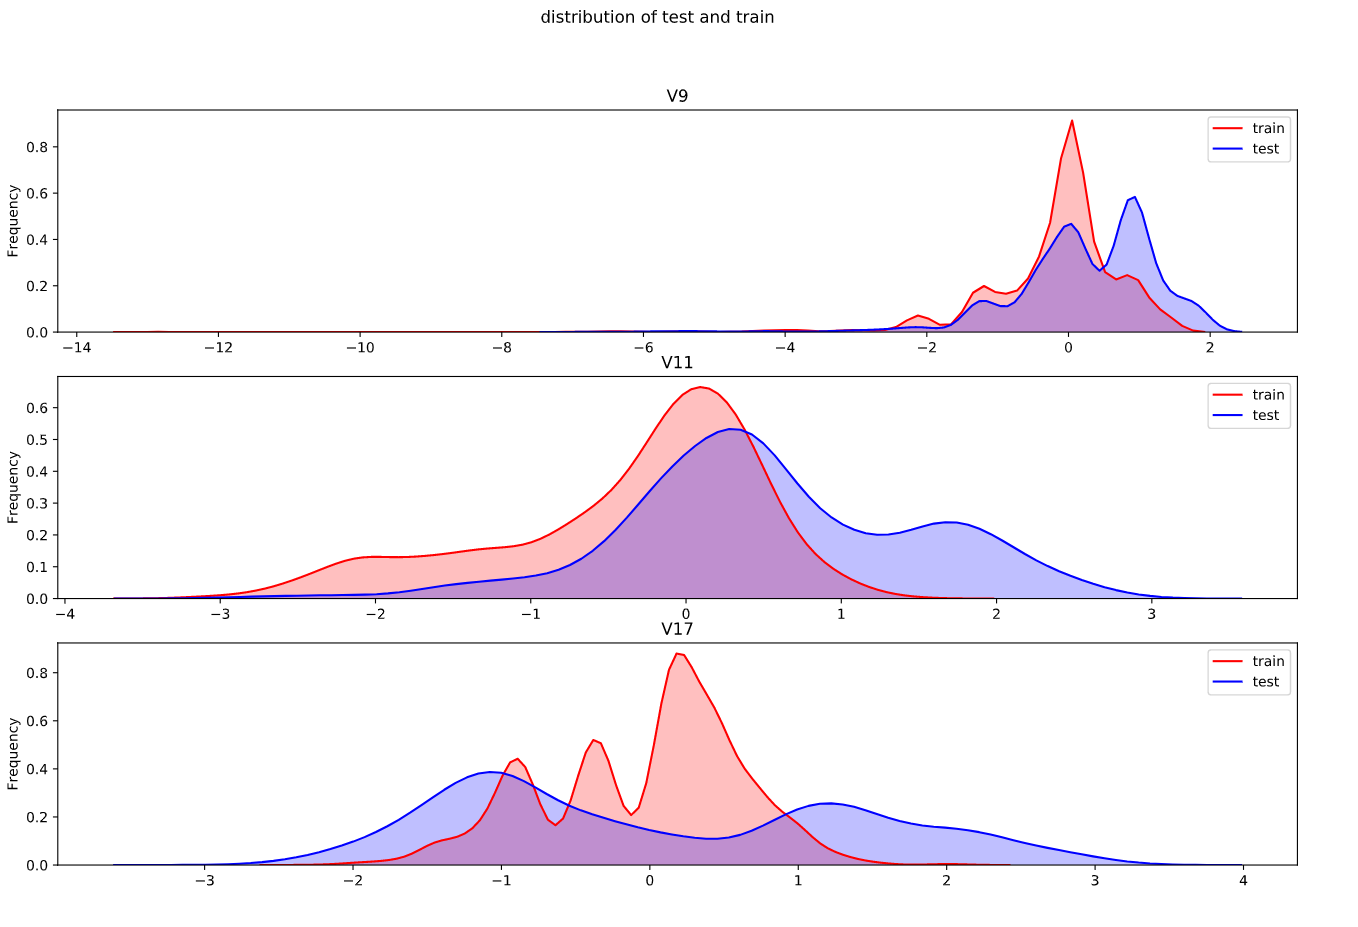
\includegraphics[width=250pt]{fig/distribution2.png}
  \caption{进一步删去的三个特征测试集与训练集差异}
  \label{fig:distri2}
\end{figure}

\subsection{模型训练}

我们通过训练不同的模型,分别输出它们的训练误差MSE,并且选取表现较好的一组做为备选方案:BayesianRidge, ElasticNetCV, LassoCV, LassoLarsCV, LinearRegression, RidgeCV, SGDRegressor, TheilSenRegressor。为了便于评估算法,首先将训练集分为两部分,分别做为算法的训练集和测试集,这样有理想的输出可以进行输出的评价。如图\ref{fig:comp}所示
\begin{figure}[htb]
  \centering
  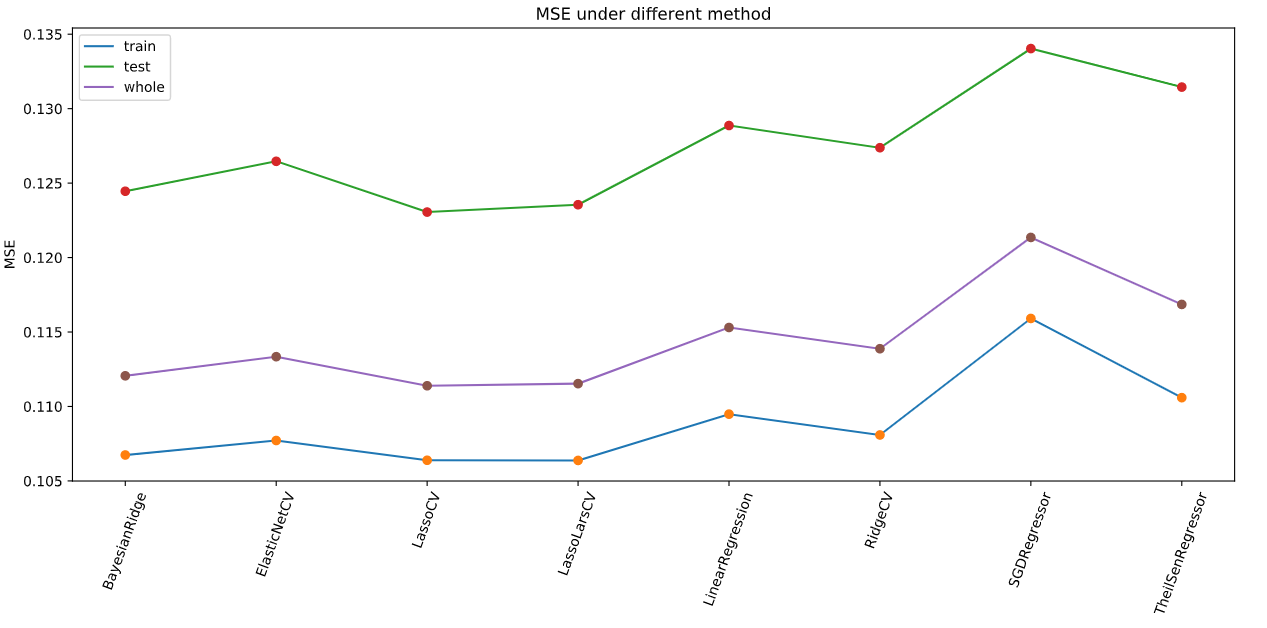
\includegraphics[width=\linewidth]{fig/comparison.png}
  \caption{不同方法在训练集上比较}
  \label{fig:comp}
\end{figure}


\subsection{评价标准}
在此数据集上进行的回归预测,采用MSE(均方误差)作为评价标准,而我们理想的结果是测试集的输出与训练集的输出稳定,这里我们引入算法稳定性判据:
$$
Stable=\begin{cases}
 & \frac{1}{\left |MSE_{test}-MSE_{train} \right |},\text{if }MSE_{test}>MSE_{train} \\ 
 & 0,\text{if }MSE_{test}<= MSE_{train}
\end{cases}
$$
其中,MSE表达式如下:
$$
M S E=\frac{1}{n} \sum (y i-\hat{y} i)^{2}
$$

\subsection{模型测试}
我们将测试集上传到官网进行测试,得出不同特征选择方法和不同模型的比较如图3:
\begin{figure}[htb]
  \centering
  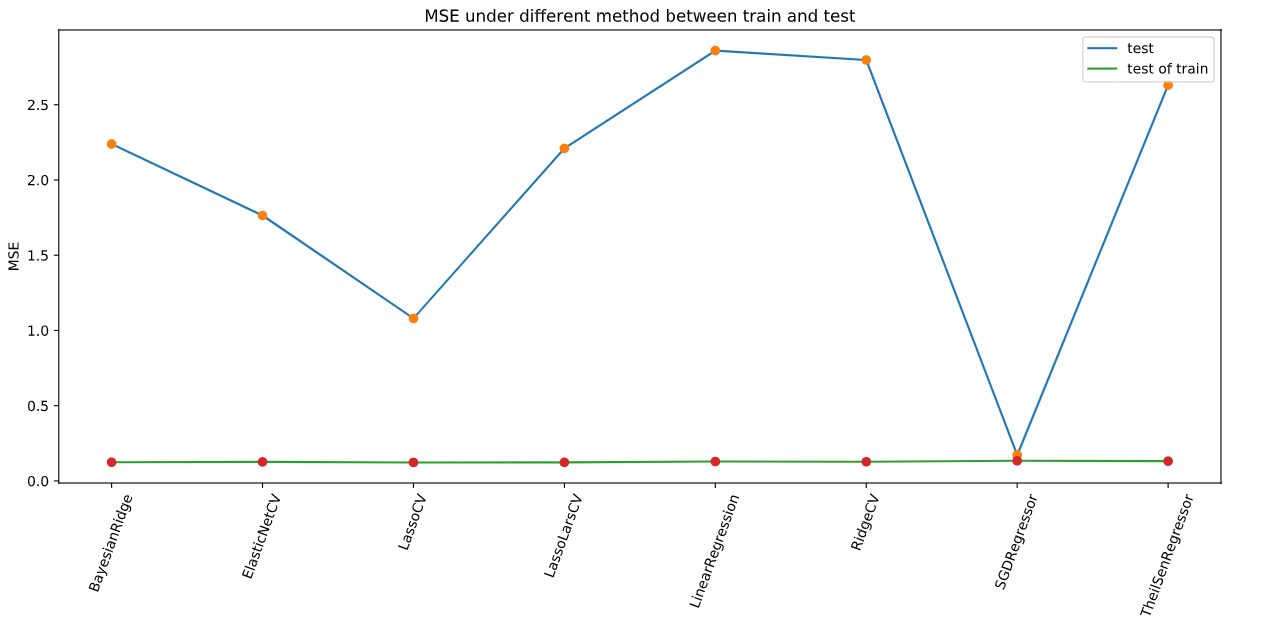
\includegraphics[width=\linewidth]{fig/comparison_test.png}
  \caption{不同方法比较}
\end{figure}
可以看出,效果最好的是 SGDRegressor, 其次是 LassoCV。于是我们下一步的主要方向是在这两个算法上进一步优化。
\section{优化}
对于该问题,我们可以想到两个方向,第一是进行模型融合,也就是利用不同的模型的优势进行优化;第二是进一步量化不同维度特征的贡献度,因为不同特征对回归结果具有差异性。
\section{结论}


\begin{table}[htb]
\begin{center}
\caption{实验结果对比}
\small
\begin{tabular}{@{}ccccc@{}}
\toprule
MSE/Stable      & SGD & XGboost& SGD + XGboost \\ \midrule
去掉两特征 & 0.1329/50.0       & 0.1219/55.6 & 0.1124/79.8   \\ \midrule \midrule
去掉五特征 & 0.1392/35.7        & 0.1258/90.9  & 0.1193/35.4 \\ \midrule
全部特征  & 0.1340/52.6       & 0.1230/58.8   & 0.1153/62.3\\ \midrule
\bottomrule
\end{tabular}
\end{center}
\end{table}
提交到线上测试集最好结果为0.1723。
\section{总结}
在测试过程中,最显著的一个问题是算法稳定性,即在训练集上表现较好的方法在测试集上并没有更好的结果,模型融合有助于提高稳定性。

\nocite{*}


% \bibliographystyle{cjc}

\addcontentsline{toc}{chapter}{参考文献}
\renewcommand{\baselinestretch}{1.6}
\begin{thebibliography}{00}

  \bibitem{AdaBoost}D. P. Solomatine and D. L. Shrestha, "AdaBoost.RT: a boosting algorithm for regression problems," 2004 IEEE International Joint Conference on Neural Networks.
 

\end{thebibliography}
% \bibliography{example}

\end{document}

